%这是LaTeX源文件
%编译要求:
%编译命令: xelatex -shell-escape rep.tex
%其他要求: 需要安装字体Bitstream Vera Sans Mono;需要安装pygments;需要文档类'cumtbrep';需要实验中用到的代码文件

\documentclass{cumtbrep}

\usepackage{float}
\usepackage{graphicx}
\usepackage{amsmath}
%hyper ref
\usepackage{hyperref}
\hypersetup{colorlinks,bookmarks=false,pdfauthor=王凌峰,pdftitle=报告4~5}
%font spec
\usepackage{fontspec}
\newfontfamily\bvsm{Bitstream Vera Sans Mono}[NFSSFamily=bvsmfamily]
%code
\usepackage{listings}
\usepackage{minted}
\setminted{breaklines,breakanywhere,mathescape,tabsize=4,style=default,fontsize=\normalsize,fontfamily=bvsmfamily,linenos}
%codes' line number format
\renewcommand{\theFancyVerbLine}{\sffamily
\textcolor[rgb]{0.5,0.5,0.5}{\scriptsize\oldstylenums{\arabic{FancyVerbLine}}}}
%listing's caption
\usepackage{caption}
\captionsetup{tablename=code}
%code with caption
\newcommand\inputcode[3][c++]{%
	\inputminted{#1}{#2}
	\begin{figure}[H]
		\centering
		\captionsetup{type=table}
		\caption{\texttt{#3}}
	\end{figure}
}
\newcommand\inline[2][c++]{\mintinline{#1}{#2}}

\begin{document}

\makeheader{计算机图形学}{王振武}{计科\numberstyle 19-2}{王凌峰}{\numberstyle 1910630221}

\namesec
\begin{enumerate}
	\setcounter{enumi}{4}\addtocounter{enumi}{-1}
	\item \hyperref[sec:4]{二维几何变换}
	\item \hyperref[sec:5]{裁剪}
\end{enumerate}

\purposesec
\noindent 选一种方法

\contentsec
\setcounter{section}{4}\addtocounter{section}{-1}
\section{二维几何变换}\label{sec:4}
把一个等腰三角形缩小为0.3倍并沿一条垂线上的中点旋转$-45^\circ$。

目录结构:{\ttfamily \lstinputlisting{../trans2d/tree}}

矩阵变换由GPU完成比较合适,因此在 \path{trivial.vert} 中声明了 \inline[glsl]{uniform mat4} 类型的变量 \inline[glsl]{M} ,表示转换矩阵。 \path{main.cc}中构造出 \inline[glsl]{M},再通过 \inline{gl::glUniformMatrix4fv} 设置vertex shader中 \inline[glsl]{M} 的值。

为了展示转换矩阵的效果,\path{trivial.vert} 中还声明了 \inline[glsl]{uniform bool} 类型的变量 \inline[glsl]{should}。\inline[glsl]{should} 为 \inline{false} 时不乘转换矩阵。
\inputcode[glsl]{../trans2d/trivial.vert}{trivial.vert}

\path{main.cc}中使用glm库完成矩阵和向量运算。在主循环里分别设置 \inline{should} 为 \inline{true} 和 \inline{false} 绘制原三角形和变换后的三角形。
\inputcode{../trans2d/main.cc}{main.cc}

\section{裁剪}\label{sec:5}
使用Liang-Barsky算法。

目录结构:{\ttfamily \lstinputlisting{../clipping/tree}}

\path{main.cc} 中画了表示窗口的矩形和一条直线的裁剪结果。
\inputcode{../clipping/main.cc}{main.cc}

主要代码在 \path{clip.cc} 中。
\inputcode{../clipping/clip.hh}{clip.hh}
\inputminted{c++}{../clipping/clip.cc}
\begin{center}
	\captionsetup{type=table}
	\caption{\texttt{clip.cc}}
\end{center}

\analysesec
\begin{figure}[H]
	\centering
	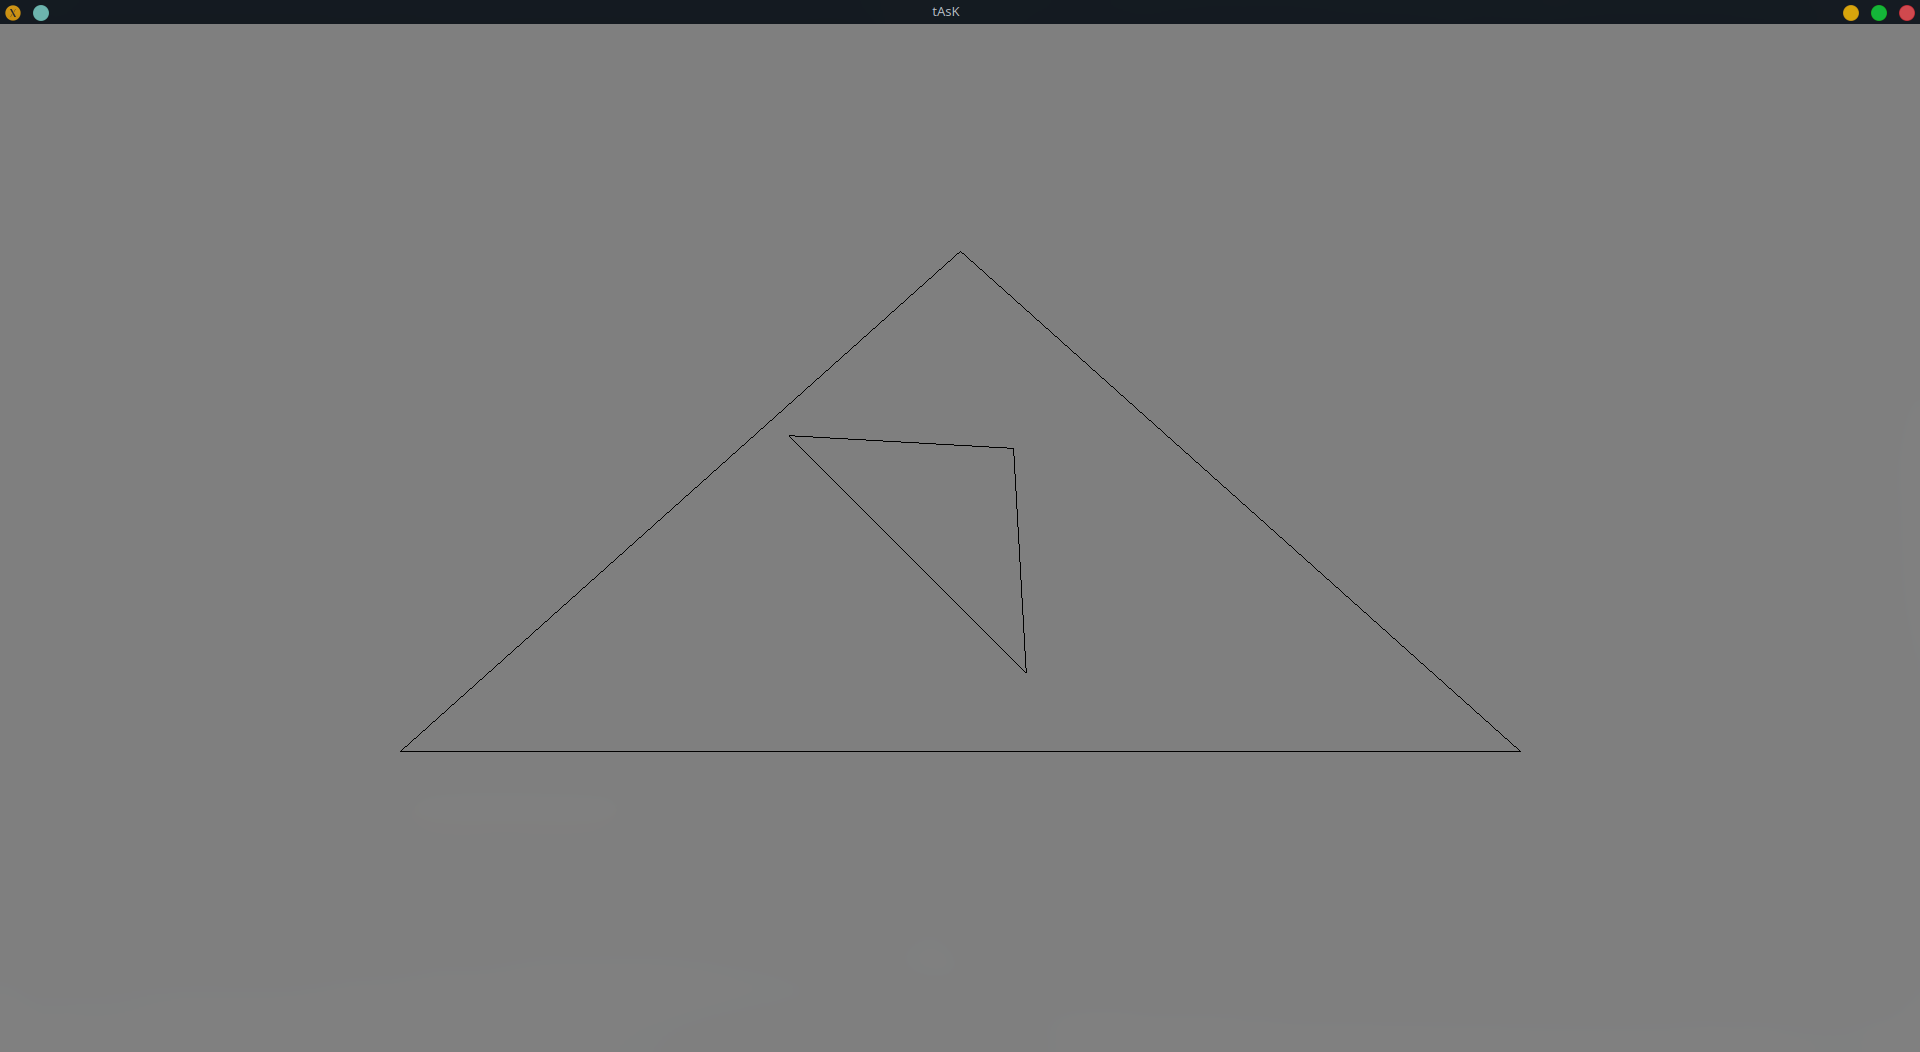
\includegraphics[scale=0.25]{../trans2d/trans2d.png}
	\caption{二维几何变换}
\end{figure}
\begin{figure}[H]
	\centering
	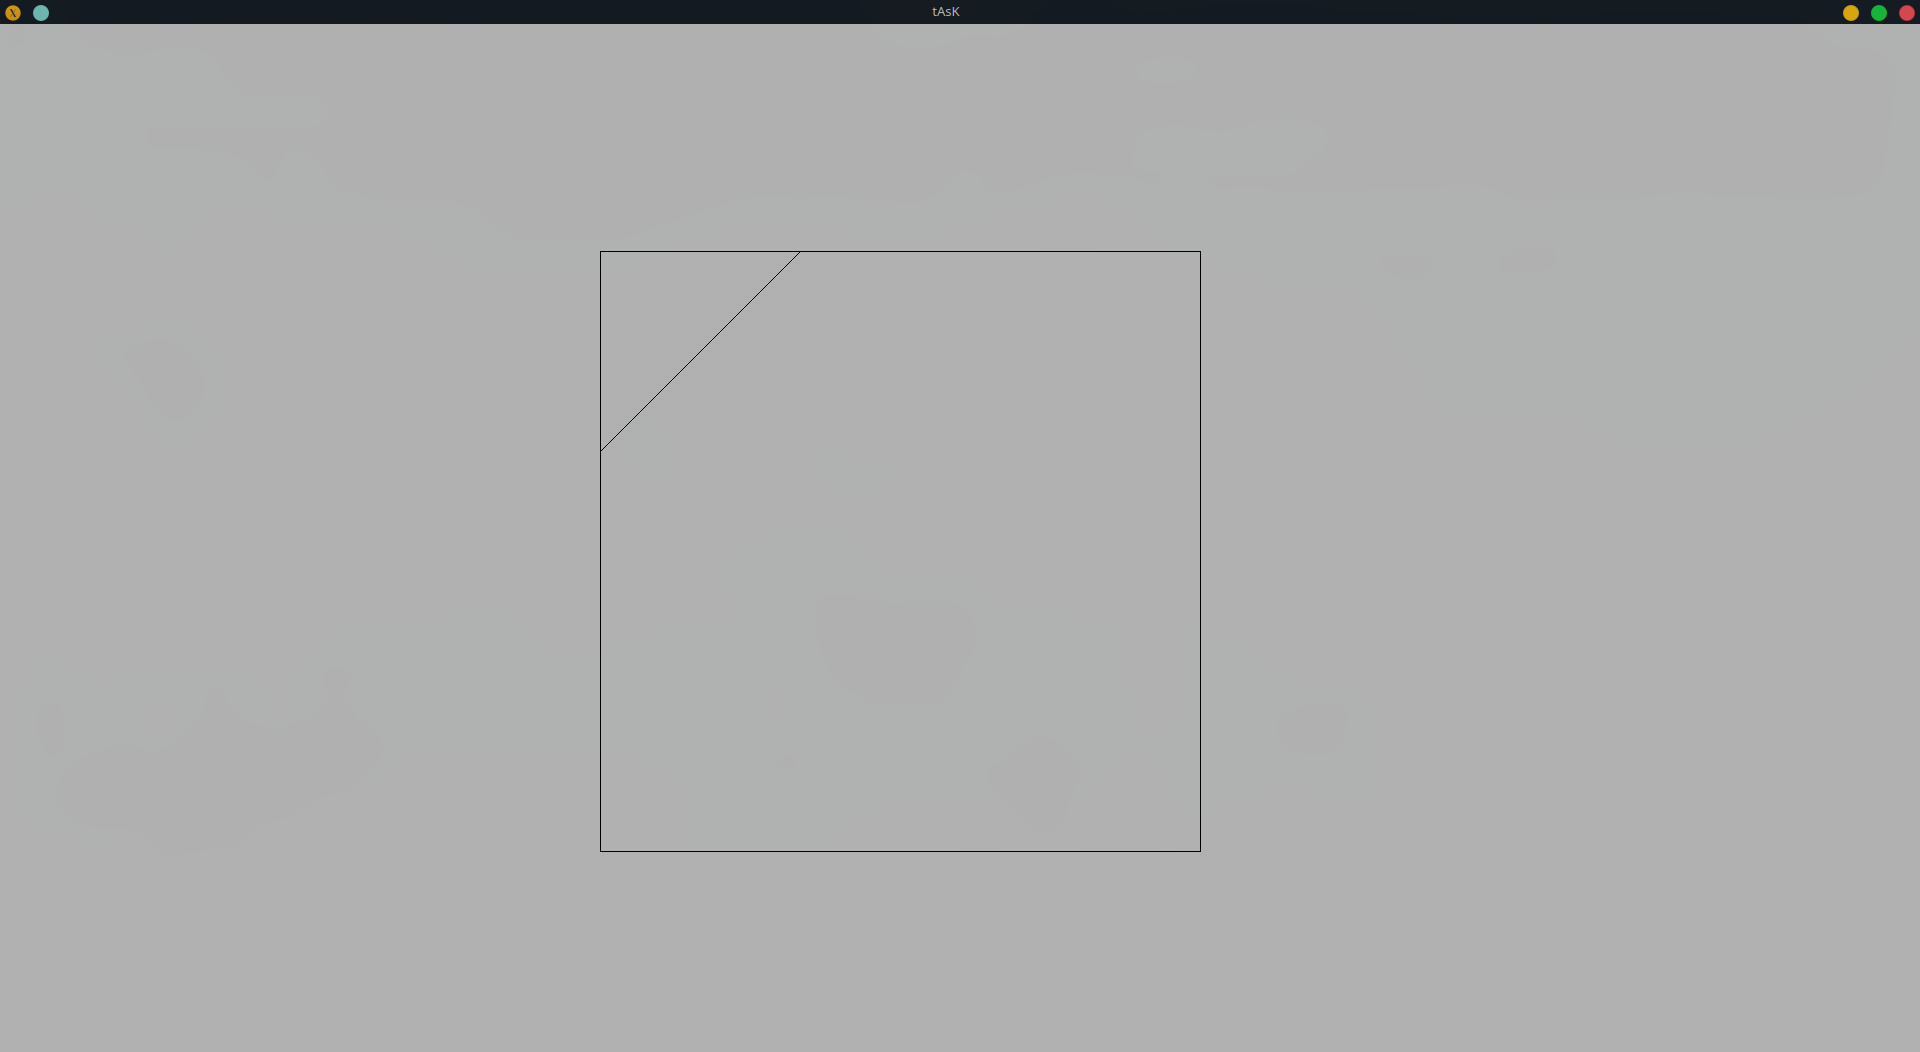
\includegraphics[scale=0.25]{../clipping/clip.png}
	\caption{二维裁剪}
\end{figure}

\maketail

\end{document}
